\chapter{Logging in our project}
% \section{Logging in our project}
\begin{figure}[hbt!]
    \centering
    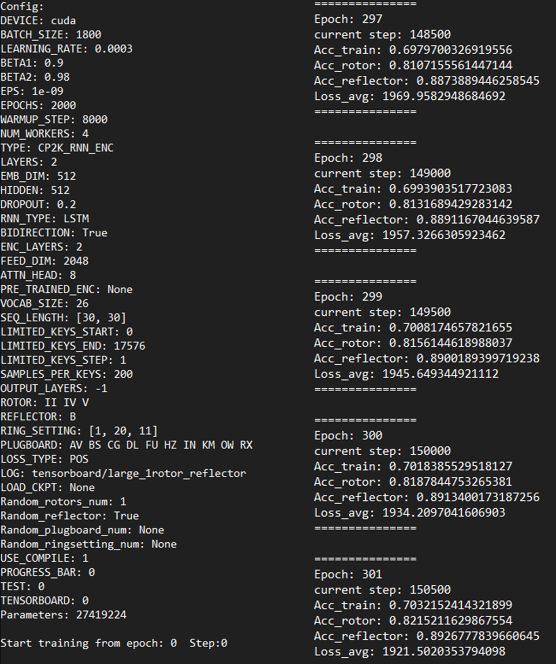
\includegraphics[width=0.7\linewidth]{myReport//figures/logfile.png}
    \caption{An output example from the log file. Left side shows all the hyper parameters used during the training. Right part of the figure tracks the results of each epoch.}
    \label{fig:enter-label}
\end{figure}

\chapter{Try out the project}
\section{Setting up the project locally}

We built entire project in an Anaconda environment, and we recommend you to do so to avoid dependencies conflict. After clone the project, you can use the bash command below to install all the requirement we needed for the project.

\begin{center}
    \\ 
    \textbf{pip install -r requirements.txt}
    \\
    \textbf{pip install tensorboard}
    \\
\end{center}

\noindent If you prefer to use Docker, you could add these line into you Dockerfile.

\section{Try out the training on Google Colab}

You can have a peek on how our project works by the Google Colab below. This notebook shows how we setting up the environment and use print and Tensorboard to trace our training results. Include the loss value, accuracy, and change of warm-up learning rate. 
This notebook is only for showcase because it would takes at least 2 to 3 hours to train the network. 

\url{https://colab.research.google.com/drive/1Ntqj5XQJFHo0qC3dB0YrHqxXu813WoQz?usp=sharing}



